% =====================================================================
% State Diagram -> Code: comprehensive IEEE-style project progress report
% Compile: pdflatex report.tex && pdflatex report.tex   (or upload to Overleaf)
% =====================================================================
\documentclass[journal,10pt]{IEEEtran}

\usepackage{cite}
\usepackage{amsmath,amssymb}
\usepackage{graphicx}
\usepackage{booktabs}
\usepackage{array}
\usepackage{xcolor}
\usepackage{url}
\usepackage{tikz}
\usetikzlibrary{positioning,arrows.meta}
\usepackage[hidelinks]{hyperref}

\graphicspath{{figures/}}
\newcommand{\code}[1]{\texttt{#1}}
\newcolumntype{L}[1]{>{\raggedright\arraybackslash}p{#1}}

\begin{document}

\title{State Diagram to Code: Reconstructing Verified State Machines from Diagram
Images --- Comprehensive Project Progress Report}

\author{[Author Name]%
\thanks{Computer Vision course project. Contact: kushagrasingh1424@gmail.com.}%
\thanks{Report date: 16 October 2026. Covers work from 14 September to 15 October 2026.}}

\markboth{Computer Vision Project Progress Report, October 2026}%
{State Diagram to Code}

\maketitle

% =====================================================================
\begin{abstract}
State-transition diagrams are usually stored as images: whiteboard photos, slides, PDFs
and textbook figures. Using one in software means re-typing it by hand, which is slow and
error-prone. This report records the full progress of a project that turns an image of a
state diagram, including computer-network protocol diagrams such as a TCP-style
handshake, into a validated machine-readable graph, lets a human correct it in a web
editor, and generates Python code that is automatically tested against that graph.

The project went through eight phases. The first prototype combined a two-class YOLO11n
detector with nearest-centre arrow linking. The current system pairs a six-class
detector with a deterministic stroke tracer that follows the ink of each arrow, Tesseract
OCR with an \emph{event [guard] / action} grammar, explicit uncertainty records, a formal
JSON schema, a sandboxed conformance-testing code generator, an optional language-model
assistant restricted to explaining and suggesting, and a human-in-the-loop correction
loop. On 360 held-out synthetic diagrams, directed transition F1 rose from 0.320 to 0.928,
endpoint accuracy from 0.614 to 0.964, initial-state accuracy from 0.000 to 0.983, and the
share of graphs that are structurally exact from 0.000 to 0.719. Generated code passed its
conformance plan on all 360 predicted graphs. An A/B/C ablation shows that the new
association algorithm and the richer detector each contribute substantially. Transition
label OCR (0.654 exact match) and the gap between synthetic and real images are the main
open problems.
\end{abstract}

\begin{IEEEkeywords}
Diagram recognition, object detection, YOLO, stroke tracing, optical character
recognition, state machines, code generation, conformance testing, human-in-the-loop.
\end{IEEEkeywords}

% =====================================================================
\section{Introduction}
% =====================================================================
\IEEEPARstart{S}{tate} machines describe UML behaviour, user-interface flows and network
protocols. Engineers draw them far more often than they write them down in
machine-readable form. Converting a drawing into code by hand is slow and error-prone,
and one wrong arrow yields code that behaves wrongly with no warning.

\subsection{Why the Task Is Hard}
The output is a \emph{graph}, not a label or a set of boxes. A correct result requires
that:
\begin{enumerate}
\item every state is found and correctly named;
\item every arrow is linked to the right \emph{source} and \emph{target}, including
arrows that cross, curve, loop back to the same state, or run in both directions between
two states;
\item every arrow label is read and split into \emph{event}, \emph{guard} and
\emph{action};
\item the initial and final states are identified.
\end{enumerate}
A single wrong endpoint or direction changes the behaviour of the generated program. The
goal is therefore to \emph{reconstruct the correct graph and say when unsure}, not merely
to detect shapes.

\subsection{Contributions}
The components built in this project are:
\begin{itemize}
\item a synthetic diagram generator that produces images, YOLO labels \emph{and} exact
ground-truth graphs;
\item a stroke-tracing association and arrow-direction algorithm;
\item a canonical JSON schema (v1.1) with a semantic graph validator;
\item a label-semantics parser with conservative network-event tagging;
\item a deterministic code generator with an independent reference semantics, a
sandboxed conformance test runner and mutation tests;
\item a graph-level evaluation framework (Hungarian matching, CER) and a threshold tuner;
\item a browser-based editor and a correction loop that turns user fixes into training
labels.
\end{itemize}
Off-the-shelf parts are YOLO11n (Ultralytics)~\cite{yolo11}, Tesseract~\cite{tesseract},
OpenCV primitives~\cite{opencv} and the Gemini API~\cite{gemini}.

\subsection{Report Outline}
Section~\ref{sec:background} gives background. Section~\ref{sec:progress} is the
detailed progress record, phase by phase. Sections~\ref{sec:system}--\ref{sec:other}
describe the system as it stands. Section~\ref{sec:data} covers data and training,
Sections~\ref{sec:results}--\ref{sec:qual} the quantitative and qualitative results, and
Sections~\ref{sec:editor}--\ref{sec:testing} the editor and software engineering. The
report closes with limitations, lessons learned, future work, and reproduction commands
in the Appendix.

% =====================================================================
\section{Background}
\label{sec:background}
% =====================================================================
\textbf{Classical line and shape detection.} Edge detection~\cite{canny} followed by the
Hough transform~\cite{hough} finds straight segments and circles in clean drawings. These
methods need hand-set thresholds, break on curves and noise, and give no semantic class.

\textbf{Learned object detection.} Single-stage detectors of the YOLO family~\cite{yolo11}
predict class-labelled bounding boxes in one pass and transfer well from pretrained
weights. For thin, elongated or curved objects such as arrows, however, an axis-aligned
box carries almost no information about endpoints or direction.

\textbf{OCR.} Tesseract~\cite{tesseract} is a widely used open-source OCR engine. It
works well on printed text but degrades on small, rotated or handwritten text, and on
crops that include parts of shape outlines.

\textbf{Language models.} Multimodal LLMs can describe a diagram or write code from it,
but their output cannot be verified pixel by pixel and is hard to measure. This project
therefore limits the LLM to explanation and suggestion, and keeps every decision that
affects correctness deterministic and testable.

\textbf{State machines.} The label notation \emph{event [guard] / action} follows UML
state machines~\cite{uml}.

% =====================================================================
\section{Project Progress}
\label{sec:progress}
% =====================================================================
This section is the core progress record. Each phase states its goal, what was built,
the problems found and the outcome. Dates come from file timestamps and the Git log.
Table~\ref{tab:commits} summarises the commits, and Table~\ref{tab:decisions} the main
design decisions.

\begin{table*}[t]
\centering
\caption{Version history of the project (Git log of \code{statetocode/})}
\label{tab:commits}
\footnotesize
\begin{tabular}{@{}llL{9.3cm}rr@{}}
\toprule
\textbf{Commit} & \textbf{Date / time} & \textbf{Summary} & \textbf{Files} & \textbf{+ / $-$ lines} \\
\midrule
--- & 14--15 Sep & Prototype (pre-Git): OpenCV dataset v1, YOLO11n v1, Hough-line and
box-merging scripts & --- & --- \\
--- & 12 Oct & Package skeleton: graph, analysis, Petri-net and network modules, first tests
& --- & --- \\
\code{d491001} & 13 Oct 11:48 & Baseline: existing pipeline before completion work & 35 &
+3260 / $-$0 \\
\code{1e84a7b} & 13 Oct 12:10 & Contract v1.1, label semantics, synthetic dataset,
stroke-tracing reconstruction, OCR, evaluation & 17 & +3139 / $-$557 \\
\code{641a4c2} & 13 Oct 12:33 & Deterministic code generation with sandboxed conformance,
Gemini suggestions, editor UI, CLI, tests & 22 & +3982 / $-$421 \\
\code{31167d2} & 13 Oct 12:46 & Self-loop and rectangle association, arrowhead exclusivity,
full-coverage conformance plans, UI fixes, TCP example, README & 16 & +1567 / $-$157 \\
\code{b7f37d7} & 13 Oct 12:51 & Record held-out evaluation results & 1 & +19 / $-$1 \\
\code{0bb60f8} & 13 Oct 13:31 & Editor: connect network devices via form or canvas; test
image generator & 6 & +367 / $-$26 \\
\code{2e06ae7} & 13 Oct 13:34 & Demo guide; deterministic demo run in generated code & 2 &
+323 / $-$4 \\
--- & 15 Oct & Presentation material: evaluation lab page, extracted detector curves,
speaker notes, slide deck & --- & --- \\
\bottomrule
\end{tabular}
\end{table*}

\subsection{Phase 0 --- First Prototype (14--15 September)}
\textbf{Goal.} Show that a detector can find the parts of a state diagram at all.

\textbf{What was built.} Three stand-alone scripts, now kept in \code{legacy/} for
comparison:
\begin{itemize}
\item \code{generate\_dataset\_v1.py} (492 lines): renders 300 diagrams of
$640\times640$\,px with OpenCV. States are circles of radius 35--55\,px at least
220\,px apart, arrows have a fixed thickness of 5\,px and a 22\,px head at
$30^\circ$. The split is 70/20/10 and the labels have two classes, \code{state} and
\code{arrow}.
\item YOLO11n v1, fine-tuned for 50 epochs (batch 16, image size 640, horizontal flip
0.5). It took about 90 minutes and reached validation mAP@50 0.994 and mAP@50--95 0.978
on this easy two-class data.
\item \code{detect\_states.py} (146 lines): a classical experiment with Gaussian blur,
Canny edges (thresholds 50/150) and probabilistic Hough lines to find arrow segments.
\item \code{postprocess\_arrows.py} (301 lines): merges fragmented arrow detections
whose centres are within 120\,px and overlap vertically by at least 30\,\%, at confidence
0.40.
\end{itemize}

\textbf{Problems found.} Hough lines only find straight segments and need per-image
thresholds. The detector often split one arrow into several boxes. Most importantly, a
box does not tell where an arrow starts or ends. The scripts were also written for
Windows with hard-coded \code{C:/statetocode} paths and a Windows virtual environment.

\textbf{Outcome.} Detection of states and arrows was feasible, but a graph could not be
built reliably. Fig.~\ref{fig:legacy} shows a post-processed output of this stage.

\begin{figure}[t]
\centering
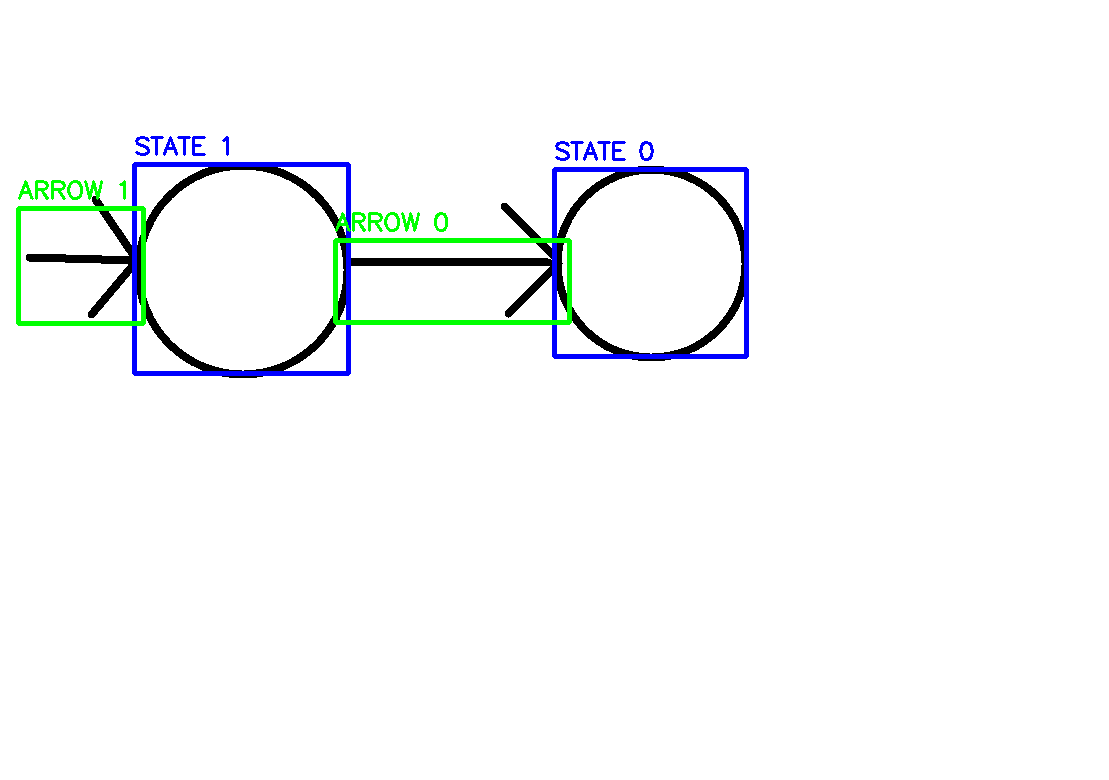
\includegraphics[width=0.8\columnwidth]{legacy_output.png}
\caption{Output of the Phase~0 prototype on the original sample image: merged arrow
boxes over the detected states.}
\label{fig:legacy}
\end{figure}

\subsection{Phase 1 --- Modular Package (12 October)}
\textbf{Goal.} Replace the loose scripts with a reusable, testable package.

\textbf{What was built.} The package \code{statemachine\_pipeline/} with a versioned JSON
contract (\code{models.py}) shared by detection, reconstruction, validation, Gemini and
code checks. It also contained a graph model and reachability/cycle analysis
(\code{graph.py}, \code{analysis.py}), a Petri-net contract with token firing
(\code{petrinet.py}), a network-topology contract with an OpenCV baseline
(\code{network.py}, \code{network\_cv.py}), a simple editor, a CLI and the first tests.
Arrows were still linked to the nearest state centre, and any label or direction the
detector could not provide stayed \code{null}/\code{unknown} with a warning instead of
being invented.

\textbf{Outcome.} The architecture was in place, but recognition quality was unchanged.

\subsection{Phase 2 --- Baseline Snapshot (13 October, \code{d491001})}
The existing pipeline (35 files, 3260 lines) was committed as a baseline so that every
later change could be measured against it. Analysis of this baseline identified the
systematic failures of nearest-centre association:
\begin{itemize}
\item \emph{invented self-loops} when both box ends were nearest the same state;
\item \emph{swapped directions}, because box corners carry no direction;
\item \emph{wrong endpoints} where edges cross;
\item no initial or final states, no OCR, and no notion of uncertainty.
\end{itemize}
This snapshot became configuration~A of the later ablation (Section~\ref{sec:results}).

\subsection{Phase 3 --- New Recognition Core (\code{1e84a7b})}
\textbf{Goal.} Reconstruct the graph from the actual strokes and read the text.

\textbf{What was built.}
\begin{itemize}
\item \textbf{Schema v1.1} with a formal JSON Schema (\code{schema.py}). It adds traced
paths, label boxes, uncertainties, provenance and network fields, and keeps 1.0 documents
loadable.
\item \textbf{Synthetic data v2} (\code{synthetic.py}, \code{generate\_dataset.py}):
2400 Pillow-rendered diagrams, six classes, exact ground-truth graph per image, generic
and network-protocol vocabularies, and photometric degradations.
\item \textbf{Ink mask} (\code{preprocess.py}) and the \textbf{stroke tracer}
(\code{arrows.py}, \code{reconstruct.py}).
\item \textbf{OCR} (\code{ocr.py}) and \textbf{label semantics} (\code{semantics.py}).
\item \textbf{Evaluation} (\code{evaluate.py}) with Hungarian matching and CER, and the
threshold \textbf{tuner} (\code{tune.py}).
\end{itemize}
The legacy scripts moved to \code{legacy/} and the YOLO11n v2 model was trained on the
new data.

\subsection{Phase 4 --- Code, Verification and Tools (\code{641a4c2})}
\textbf{Goal.} Make the graph usable and its code trustworthy.

\textbf{What was built.} The deterministic template code generator with a separate
reference semantics and test-plan builder (\code{codegen.py}), the sandbox
(\code{sandbox.py}) and trace replay (\code{trace.py}), the Gemini backend with
contract checks and accept/reject suggestions (\code{gemini.py}), the correction store
and YOLO export (\code{corrections.py}), the full web editor (\code{ui.py},
\code{static/}), the complete CLI (\code{main.py}) and the bulk of the test suite.

\subsection{Phase 5 --- Hard Cases (\code{31167d2})}
\textbf{Goal.} Fix the error classes that remained after Phase~3.

\textbf{What changed.}
\begin{itemize}
\item \textbf{Self-loops and rounded rectangles:} a trace that leaves a state's region
and comes back to it is now a self-loop, and state regions handle rectangular outlines.
\item \textbf{Arrowhead exclusivity:} each detected arrowhead may belong to only one
arrow, which separates two nearly parallel curved arrows.
\item \textbf{Full-coverage conformance plans:} transitions out of states that cannot be
reached from the initial state are now also exercised, by starting the trace at their
source state.
\item A complete worked example (\code{examples/tcp\_like/}: image, JSON, code, tests and
report), UI fixes, and a full README rewrite.
\end{itemize}

\subsection{Phase 6 --- Held-out Evaluation (\code{b7f37d7})}
The three configurations A, B and C were evaluated on the 360-image test split, which had
never been used for training or tuning, and the results were recorded in the README and
\code{outputs/comparison.md} (Table~\ref{tab:ablation}).

\subsection{Phase 7 --- Network Editing and Demo (\code{0bb60f8}, \code{2e06ae7})}
The editor gained network-device and link editing, either through a form or by clicking
two devices on the canvas, and duplicate links are refused. \code{make\_test\_images.py}
generates 35 fixed-seed demo images in five groups: generic, network protocol, hard
cases, photo-like and topology. \code{DEMO.md} is a scripted 15-minute live demo, and the
generated code gained a deterministic demonstration run.

\subsection{Phase 8 --- Presentation Material (15 October)}
\code{demo/extract\_curves.py} extracts the detector's precision-recall and confidence
curves, per-class metrics and confusion matrix into \code{evaluation\_data.json}. These
feed an interactive evaluation page (\code{evaluation\_lab.html}), a slide deck
(\code{state\_diagram\_to\_code.pptx}) and speaker notes.

\subsection{Progress Summary}
The project grew from three scripts (about 940 lines) to a package of about 8.6k lines of
Python and JavaScript across 24 modules, a static front-end, 11 test files and the CLI.
Table~\ref{tab:before-after} compares the first and current versions.

\begin{table}[t]
\centering
\caption{First version versus current version}
\label{tab:before-after}
\footnotesize
\begin{tabular}{@{}L{2.0cm}L{2.7cm}L{3.0cm}@{}}
\toprule
\textbf{Aspect} & \textbf{Phase 0 / baseline} & \textbf{Current} \\
\midrule
Classes & 2 & 6 \\
Training data & 300 OpenCV images & 2400 Pillow images + graph truth \\
Association & Nearest state centre & Stroke tracing, both ends \\
Direction & None (box order) & Arrowhead + headness, exclusive \\
Initial/final & None & Marker, double ring, classes \\
Text & None & Tesseract + label grammar \\
Uncertainty & None & Explicit records, editor highlight \\
Validation & Basic & JSON Schema + 7 graph rules \\
Code & Gemini + syntax checks & Template + reference + sandbox \\
Evaluation & mAP only & Graph-level metrics, ablation \\
Transition F1 & 0.320 & 0.928 \\
Tests & 3 files & 70 test functions in 11 files \\
\bottomrule
\end{tabular}
\end{table}

\begin{table*}[t]
\centering
\caption{Key design decisions and their rationale}
\label{tab:decisions}
\footnotesize
\begin{tabular}{@{}L{4.2cm}L{12.6cm}@{}}
\toprule
\textbf{Decision} & \textbf{Reason} \\
\midrule
Trace strokes instead of linking to nearest centre & Boxes carry no connectivity;
nearest-centre linking invents self-loops, swaps directions and fails at crossings
(transition F1 0.32 vs 0.59 on the same detector). \\
Six detector classes & Arrowheads give direction evidence; initial markers, final states
and labels each needed their own signal (F1 0.59 $\rightarrow$ 0.93). \\
Synthetic training data & Unlimited, perfectly labelled data \emph{with exact graph
truth}, enabling whole-graph evaluation; the domain gap is stated as a limitation. \\
Horizontal flip disabled & Mirrored text never occurs in real diagrams; a design choice,
not ablated. \\
Hungarian matching on IoU & Output IDs are detection order; an optimal one-to-one
assignment is required for fair scoring. \\
Deterministic code generation & Behaviour must be exact and testable; the LLM is an
optional, checked alternative. \\
Report uncertainty, do not guess & A silent guess produces wrong code without warning;
uncertain items are handed to the user. \\
Standard-library HTTP server & No framework dependency for a local tool; bound to
127.0.0.1 with upload checks. \\
Learned perception, deterministic reasoning & Each tool does what it is good at; the
reasoning steps are explainable, debuggable and need no extra labelled data. \\
\bottomrule
\end{tabular}
\end{table*}

% =====================================================================
\section{System Overview}
\label{sec:system}
% =====================================================================
Fig.~\ref{fig:pipeline} shows the current pipeline. The guiding principle is that
\emph{learned components perceive and deterministic components reason}. A neural network
decides what is where, classical image processing decides what connects to what, and
validators and tests decide whether the graph and the code are acceptable. The language
model only explains and suggests.

\begin{figure}[t]
\centering
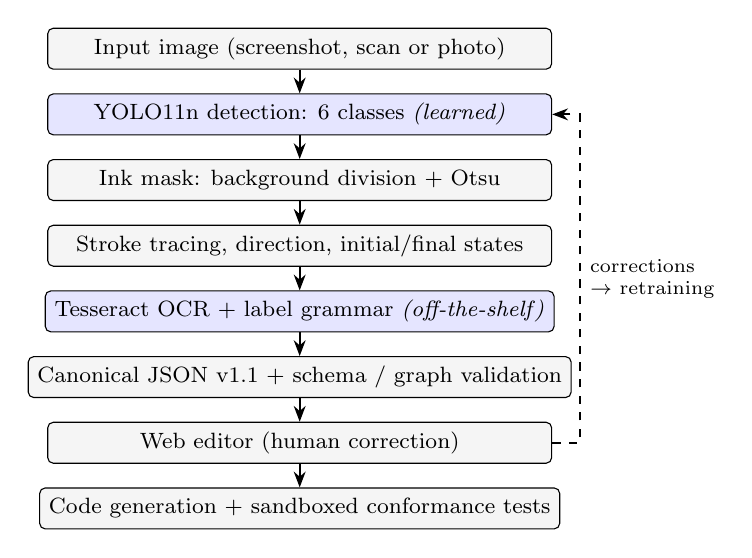
\begin{tikzpicture}[
  node distance=0.30cm,
  box/.style={draw, rounded corners=2pt, align=center, font=\footnotesize,
              minimum width=6.4cm, minimum height=0.52cm, fill=gray!8},
  lrn/.style={box, fill=blue!10},
  arr/.style={-{Stealth[length=2mm]}, thick}]
\node[box] (img) {Input image (screenshot, scan or photo)};
\node[lrn, below=of img] (det) {YOLO11n detection: 6 classes \textit{(learned)}};
\node[box, below=of det] (ink) {Ink mask: background division + Otsu};
\node[box, below=of ink] (trc) {Stroke tracing, direction, initial/final states};
\node[lrn, below=of trc] (ocr) {Tesseract OCR + label grammar \textit{(off-the-shelf)}};
\node[box, below=of ocr] (json) {Canonical JSON v1.1 + schema / graph validation};
\node[box, below=of json] (ed) {Web editor (human correction)};
\node[box, below=of ed] (code) {Code generation + sandboxed conformance tests};
\draw[arr] (img) -- (det);
\draw[arr] (det) -- (ink);
\draw[arr] (ink) -- (trc);
\draw[arr] (trc) -- (ocr);
\draw[arr] (ocr) -- (json);
\draw[arr] (json) -- (ed);
\draw[arr] (ed) -- (code);
\draw[arr, dashed] (ed.east) -- ++(0.35,0) |- node[pos=0.25, right, font=\scriptsize,
  align=left]{corrections\\$\rightarrow$ retraining} (det.east);
\end{tikzpicture}
\caption{Processing pipeline. Blue stages are learned or off-the-shelf models; the rest is
deterministic. The dashed path is the human-in-the-loop correction loop. Gemini (not
shown) attaches to the editor for explanation and suggestions only.}
\label{fig:pipeline}
\end{figure}

\begin{table}[t]
\centering
\caption{Pipeline stages and modules}
\label{tab:modules}
\footnotesize
\begin{tabular}{@{}lll@{}}
\toprule
\textbf{Stage} & \textbf{Module} & \textbf{Technique} \\
\midrule
Detection & \code{detector.py} & YOLO11n \\
Ink segmentation & \code{preprocess.py} & Background division, Otsu \\
Association & \code{arrows.py}, & Direction-following tracer \\
 & \code{reconstruct.py} & \\
Direction & \code{arrows.py} & Arrowhead box + headness \\
Text & \code{ocr.py} & Tesseract + glyph clean-up \\
Label meaning & \code{semantics.py} & Grammar + keyword table \\
Validation & \code{validation.py} & JSON Schema + graph rules \\
Analysis & \code{analysis.py} & Reachability, cycles, dead ends \\
Code generation & \code{codegen.py} & Template or Gemini \\
Verification & \code{sandbox.py}, & Isolated conformance tests \\
 & \code{trace.py} & \\
\bottomrule
\end{tabular}
\end{table}

\textbf{Tech stack.} Python~3 throughout; Ultralytics YOLO11n (PyTorch); OpenCV and NumPy
for image processing; SciPy for the Hungarian algorithm; Tesseract via pytesseract
(optional); jsonschema; Pillow for rendering; \code{google-genai} for Gemini (optional);
the standard-library \code{http.server} with plain HTML/JavaScript for the editor; and
pytest. Missing Tesseract or a missing Gemini key degrades the system gracefully and does
not break it.

% =====================================================================
\section{Computer-Vision Pipeline}
\label{sec:cv}
% =====================================================================

\subsection{Object Detection}
YOLO11n, the nano variant of YOLO11, detects six classes: \code{state}, \code{arrow},
\code{final\_state}, \code{arrowhead}, \code{initial\_marker} and \code{label}. The inputs
are simple line drawings, so the smallest model is enough; it runs on a laptop GPU or a
CPU. Detection runs at a confidence threshold of 0.40. The detector alone cannot solve the
task. The box of a curved or diagonal arrow covers a large area, overlaps other objects,
and says nothing about where the arrow starts, ends or points.

\subsection{Ink Mask}
The stroke analysis needs a binary ink image that also works on shaded photos:
\begin{enumerate}
\item estimate the background with a large morphological closing, which removes thin dark
lines but keeps paper shading;
\item divide the image by the background, which flattens shadows and gradients;
\item apply a light Gaussian blur and Otsu thresholding~\cite{otsu};
\item remove speckle with a small morphological opening.
\end{enumerate}
The pen width is estimated from the distance transform: the median distance on the stroke
centre-line is half the width, and the tracer scales its tolerances by it. CLAHE~\cite{clahe}
on the L channel of LAB is available for faint images.

\subsection{Stroke-Tracing Association}
This algorithm is the main technical contribution of the project.
\begin{enumerate}
\item \textbf{State regions.} Each state box is grown until its outline ink ends
(padding of $\max(3\,\text{px}, 0.1\times\text{size})$) and the region is removed from the
mask, leaving only free strokes.
\item \textbf{Ports.} A port is where ink crosses a thin ring (3\,px) just outside a state,
i.e.\ a point where an arrow leaves or enters.
\item \textbf{Tracing.} From each port the tracer advances in 2\,px steps. At every step
it searches within $\pm50^\circ$ of its heading for a direction whose ink fraction is at
least 0.5. Candidate directions are scored by ink with a small turning penalty
(\code{straight\_bias} $=0.004$ per degree). Because of this the tracer
(a)~passes straight through crossings instead of turning onto the other edge,
(b)~follows curves, since turning is only penalised, and
(c)~bridges gaps of up to 14\,px plus the stroke width, e.g.\ where a label is drawn over
the line.
\item \textbf{Termination.} A trace stops when it enters another state (an edge), when it
re-enters its own state after leaving its region (a self-loop), or when it runs out of ink
(a free end, kept only if longer than 18\,px).
\item \textbf{Cross-checking.} Every arrow is traced from both ends. Traces whose endpoints
agree within 14\,px are merged; a one-sided trace is marked uncertain. A candidate path
that overlaps already accepted arrows by more than 40\,\% is rejected, which removes
mis-traces at crossings.
\end{enumerate}

Table~\ref{tab:params} lists all 13 parameters of the tracer.

\begin{table}[t]
\centering
\caption{Tracer parameters (\code{DEFAULT\_CONFIG}); $^\ast$ = tuned on the validation split}
\label{tab:params}
\footnotesize
\begin{tabular}{@{}llL{3.6cm}@{}}
\toprule
\textbf{Parameter} & \textbf{Value} & \textbf{Meaning} \\
\midrule
\code{step} & 2 px & Tracer step length \\
\code{max\_turn\_deg} & 50$^\circ$ & Search cone half-angle \\
\code{straight\_bias}$^\ast$ & 0.004 & Penalty per degree of turn \\
\code{min\_ink\_fraction} & 0.5 & Ink needed to continue \\
\code{bridge\_gap} & 14 px & Largest gap bridged (+ width) \\
\code{port\_ring} & 3 px & Ring width for port detection \\
\code{region\_pad\_min} & 3 px & Minimum state-region padding \\
\code{region\_pad\_ratio} & 0.1 & Relative state-region padding \\
\code{min\_free\_length} & 18 px & Shortest free end kept \\
\code{endpoint\_tolerance}$^\ast$ & 14 px & Merge distance of two traces \\
\code{overlap\_reject}$^\ast$ & 0.4 & Max overlap with accepted paths \\
\code{head\_ratio}$^\ast$ & 2.2 & Headness meaning ``arrowhead'' \\
\code{direction\_margin}$^\ast$ & 0.25 & Needed headness difference \\
\bottomrule
\end{tabular}
\end{table}

\subsection{Arrow Direction}
Direction decides which state is the source and which the target, so it needs evidence:
\begin{itemize}
\item \textbf{Main evidence:} a detected \code{arrowhead} box at the arrow's own end
segment.
\item \textbf{Fallback (headness):} the ink cross-section width near each end of the
traced path divided by the shaft width. It is about 1.0 at a plain end and at least 2 at
a head (\code{head\_ratio} $=2.2$). The end that is higher by at least
\code{direction\_margin} is the head.
\item \textbf{Exclusivity:} each arrowhead can belong to only one arrow, which resolves
shallow crossings between two parallel curved arrows.
\item \textbf{Weak evidence:} the direction is set to \code{unknown} and both readings
are stored as an uncertainty. The system never guesses silently.
\end{itemize}

\subsection{Initial and Final States, Shape}
An arrow with a free tail whose head touches a state is the \emph{initial marker} (an
entry arrow or a UML black dot); a detected \code{initial\_marker} box next to a state is
the fallback. If there are several candidates, the most confident wins and the others are
reported. A \emph{final} state comes from the \code{final\_state} class or from a double
ring found in a radial ink profile: the fraction of 90 sampled angles that hit ink at
each relative radius, where two rings separated by a gap mean a double outline. Circle
versus rounded rectangle is decided by whether the box diagonals carry ink near the
corners.

\subsection{Text Reading}
For state names, the interior of each state is cropped, upscaled two to three times and
binarised with Otsu. Outline fragments are then removed (components that touch the crop
border or span most of it), because Tesseract otherwise reads the circle as ``\code{|}''
or quotes. Each transition label is assigned to the transition whose \emph{traced path} is
nearest, not whose centre is nearest. A label about equally close to two transitions, or
OCR confidence below 0.6, creates an uncertainty. If the detector has no \code{label}
class, text boxes are found from connected components.

\subsection{Label Semantics}
Labels follow the UML pattern \emph{event [guard] / action}~\cite{uml}, e.g.\
\code{timeout [retries<3] / retransmit}, and are parsed with a small grammar. Words from
an explicit keyword table (SYN, ACK, FIN, timeout, retry, connect, disconnect, failure,
send, receive, \dots) mark the transition as a \emph{network event} with an event type and
protocol. Unknown words stay plain events, so no protocol behaviour is invented.

\subsection{Uncertainty Reporting}
Every ambiguous decision creates an \code{uncertainty} record with the element, field,
reason and candidate interpretations. A dangling arrow does not create a transition; it
raises a warning that a state may be missing. The editor draws uncertain elements in
amber with dashed lines and invalid ones in red.

% =====================================================================
\section{Data Model and Validation}
\label{sec:model}
% =====================================================================
Every component uses one canonical JSON format, schema version 1.1, defined in
\code{models.py} with a formal JSON Schema in \code{schema.py}. Version 1.0 documents still
load. Table~\ref{tab:json} lists its main parts.

\begin{table}[t]
\centering
\caption{Canonical JSON (schema 1.1)}
\label{tab:json}
\footnotesize
\begin{tabular}{@{}L{1.8cm}L{6.0cm}@{}}
\toprule
\textbf{Concept} & \textbf{Fields} \\
\midrule
State & id, label, type (initial/normal/final), position, bbox, shape, confidences,
provenance \\
Transition & source, target, event, guard, action, raw label, direction, traced
\code{points}, \code{label\_bbox}, confidence, provenance \\
Network event & \code{kind = "network\_event"}, \code{network: \{event\_type, protocol,
packet\}} \\
Topology & \code{network.devices[]} (with owned states), \code{network.links[]} \\
Uncertainty & element, field, reason, candidate interpretations \\
Provenance & source image (path, size, SHA-256), per-element provenance,
\code{metadata.warnings} \\
\bottomrule
\end{tabular}
\end{table}

\code{validate\_state\_machine} first checks the JSON Schema, which rejects unknown fields
and bad values, and then applies graph rules: (1)~dangling references, (2)~duplicate IDs,
(3)~at most one initial state, (4)~non-determinism, (5)~transitions out of final states,
(6)~unreachable states, and (7)~unknown devices or links. Malformed input gives errors,
not crashes. Every editor save and every code generation is validated, and the round trip
\code{StateMachine.from\_dict(json) == machine} is tested. Because the graph view, the
JSON tab and the code are all views of this one file, they cannot drift apart.
\code{analysis.py} additionally reports reachability, cycles, dead ends and network-event
summaries.

% =====================================================================
\section{Code Generation and Verification}
\label{sec:codegen}
% =====================================================================

\subsection{Template Generator}
The default generator (\code{codegen.py}) is deterministic. It writes a dependency-free
Python \code{StateMachine} class with defined semantics:
\begin{itemize}
\item an event-less transition is triggered by its ID;
\item guards are injected callables, and a missing implementation raises
\code{GuardNotImplementedError};
\item there are explicit errors \code{InvalidEventError}, \code{GuardRejectedError},
\code{TerminalStateError} (events in final states) and
\code{NondeterministicTransitionError};
\item action hooks run \emph{before} the state changes, and network-event metadata is kept
per transition.
\end{itemize}
A machine with no initial state starts in the first state, and the code documents this.
Typical use of the generated class:

{\footnotesize
\begin{verbatim}
from tcp_machine import StateMachine
m = StateMachine(guards={
  "retries< 3": lambda c: c["retries"] < 3,
  "retries>=3": lambda c: c["retries"] >= 3})
m.submit("connect")                 # 'S1'
m.submit("timeout", {"retries": 1}) # stays S1
m.submit("timeout", {"retries": 3}) # back to S0
m.submit("ACK")                     # InvalidEventError
\end{verbatim}
}

\subsection{Conformance Testing}
The same semantics are implemented a second time, independently, as a reference model
(\code{reference\_step}). From the graph a test plan is built that fires \emph{every}
transition, starting from the initial state if the transition is reachable and from its
source state otherwise, and adds guard-rejection and invalid-event probes. The generated
code must produce exactly the same state sequence and the same errors as the reference.
The plan can be exported as a stand-alone pytest module (\code{--tests}), and single event
traces can be replayed with \code{verify}. Mutation tests confirm that deliberately broken
code is caught.

\subsection{Sandbox}
Generated code, including Gemini's, is executed in a separate interpreter:
\begin{itemize}
\item started with \code{-I -S} (isolated mode, no site packages), an empty environment and
a temporary working directory;
\item with a timeout and resource limits: 5\,s CPU, 768\,MB address space, 1\,MB file
size, 64 processes;
\item with an audit hook that blocks sockets, subprocesses, \code{os.system}/\code{exec}/
\code{spawn}, file writes and deletes, and \code{ctypes};
\item after a static AST allowlist check that rejects imports such as \code{os},
\code{socket} and \code{subprocess} and calls to \code{open}, \code{eval} and \code{exec}.
\end{itemize}
This is defence in depth for a local tool, not a hardened container.

% =====================================================================
\section{Role of the Language Model}
\label{sec:llm}
% =====================================================================
Gemini~\cite{gemini} is optional. It requires \code{GEMINI\_API\_KEY}, and the model name
comes from \code{GEMINI\_MODEL}. Table~\ref{tab:gemini} lists what it may do and how each
output is checked. It never detects arrows, validates graphs or accepts code.

\begin{table}[t]
\centering
\caption{Gemini capabilities and safeguards}
\label{tab:gemini}
\footnotesize
\begin{tabular}{@{}L{2.2cm}L{5.6cm}@{}}
\toprule
\textbf{Capability} & \textbf{Safeguard} \\
\midrule
Explain the diagram & JSON contract; explanations that mention non-existent states or
transitions are dropped \\
Suggest corrections & Each suggestion validated; shown with Accept/Reject; never applied
automatically \\
Alternative code backend & Same AST check, sandbox and conformance plan as template code \\
Propose test cases & Replayed on the reference model and marked agree/disagree \\
Failure / no key & Clear error; the rest of the system is unaffected \\
\bottomrule
\end{tabular}
\end{table}

% =====================================================================
\section{Other Diagram Types}
\label{sec:other}
% =====================================================================
\textbf{Network topology.} Diagrams of components drawn as circles joined by lines use a
separate contract, \code{network-1.0} (\code{--diagram-type network}). An OpenCV baseline
(\code{network\_cv.py}) detects circular components and connecting strokes and optionally
reads labels with OCR. Dangling edges are rejected by the contract. A generator
(\code{generate\_network\_diagrams.py}) produces samples with ground truth, and the editor
switches to a topology mode for these files.

\textbf{Petri nets.} \code{petrinet.py} defines places, transitions, weighted arcs and an
initial marking, validates dangling arcs, and implements token firing; firing a disabled
transition is rejected. Detection requires a separately trained model with classes
\code{place}, \code{transition} and \code{arc}, which has not been trained yet.

% =====================================================================
\section{Data and Training}
\label{sec:data}
% =====================================================================

\subsection{Synthetic Dataset v2}
Labelling thousands of real diagrams by hand is impractical, so diagrams are rendered
programmatically. Each sample yields the image, YOLO labels \emph{and} the exact
ground-truth graph, which makes it possible to score the whole reconstruction and not only
the boxes. The generator varies:
\begin{itemize}
\item state shape: circles, rounded rectangles, double-circle final states;
\item initial markers: plain entry arrow or UML filled dot;
\item edges: straight, curved, crossing, bidirectional pairs, self-loops;
\item labels: UML \emph{event [guard] / action} with generic or network-protocol
vocabularies;
\item degradations: line-width jitter, blur, noise and JPEG artefacts.
\end{itemize}
2400 images were generated (seed 7) and split 70/15/15 into 1680 training, 360
validation and 360 test images. The test split is used only for final results.
Table~\ref{tab:data} compares v1 and v2.

\begin{table}[t]
\centering
\caption{Datasets and training configuration}
\label{tab:data}
\footnotesize
\begin{tabular}{@{}lcc@{}}
\toprule
 & \textbf{v1 (Phase 0)} & \textbf{v2 (current)} \\
\midrule
Renderer & OpenCV & Pillow \\
Images & 300 & 2400 \\
Split (train/val/test) & 70/20/10\,\% & 1680/360/360 \\
Classes & 2 & 6 \\
Ground-truth graph & no & yes \\
Labels / photometric noise & no / no & yes / yes \\
Init. weights & \code{yolo11n.pt} & \code{yolo11n.pt} \\
Epochs & 50 & 60 (patience 15) \\
Batch / image size & 16 / 640 & 16 / 640 \\
Horizontal flip & 0.5 & 0.0 \\
Training time & $\approx$90 min & $\approx$9 min (GPU) \\
Final val.\ mAP@50 & 0.994 & 0.995 \\
Final val.\ mAP@50--95 & 0.978 & 0.933 \\
\bottomrule
\end{tabular}
\end{table}

\subsection{Detector Training}
The v2 detector was fine-tuned from pretrained \code{yolo11n.pt} weights with the
optimiser chosen automatically by Ultralytics (initial learning rate 0.01, 3 warm-up
epochs). Horizontal flipping was disabled because a mirrored diagram has mirrored text,
which never occurs in real diagrams. All 60 epochs ran, since early stopping never
triggered. Validation loss stays close to training loss and mAP levels off, so there is no
sign of overfitting (Fig.~\ref{fig:training}). At the last epoch the validation split gave
precision 0.997, recall 0.988, mAP@50 0.995 and mAP@50--95 0.933. The v1 model's higher
mAP@50--95 (0.978) is not comparable: it was measured on a much easier two-class task
with large objects only.

\begin{figure}[t]
\centering
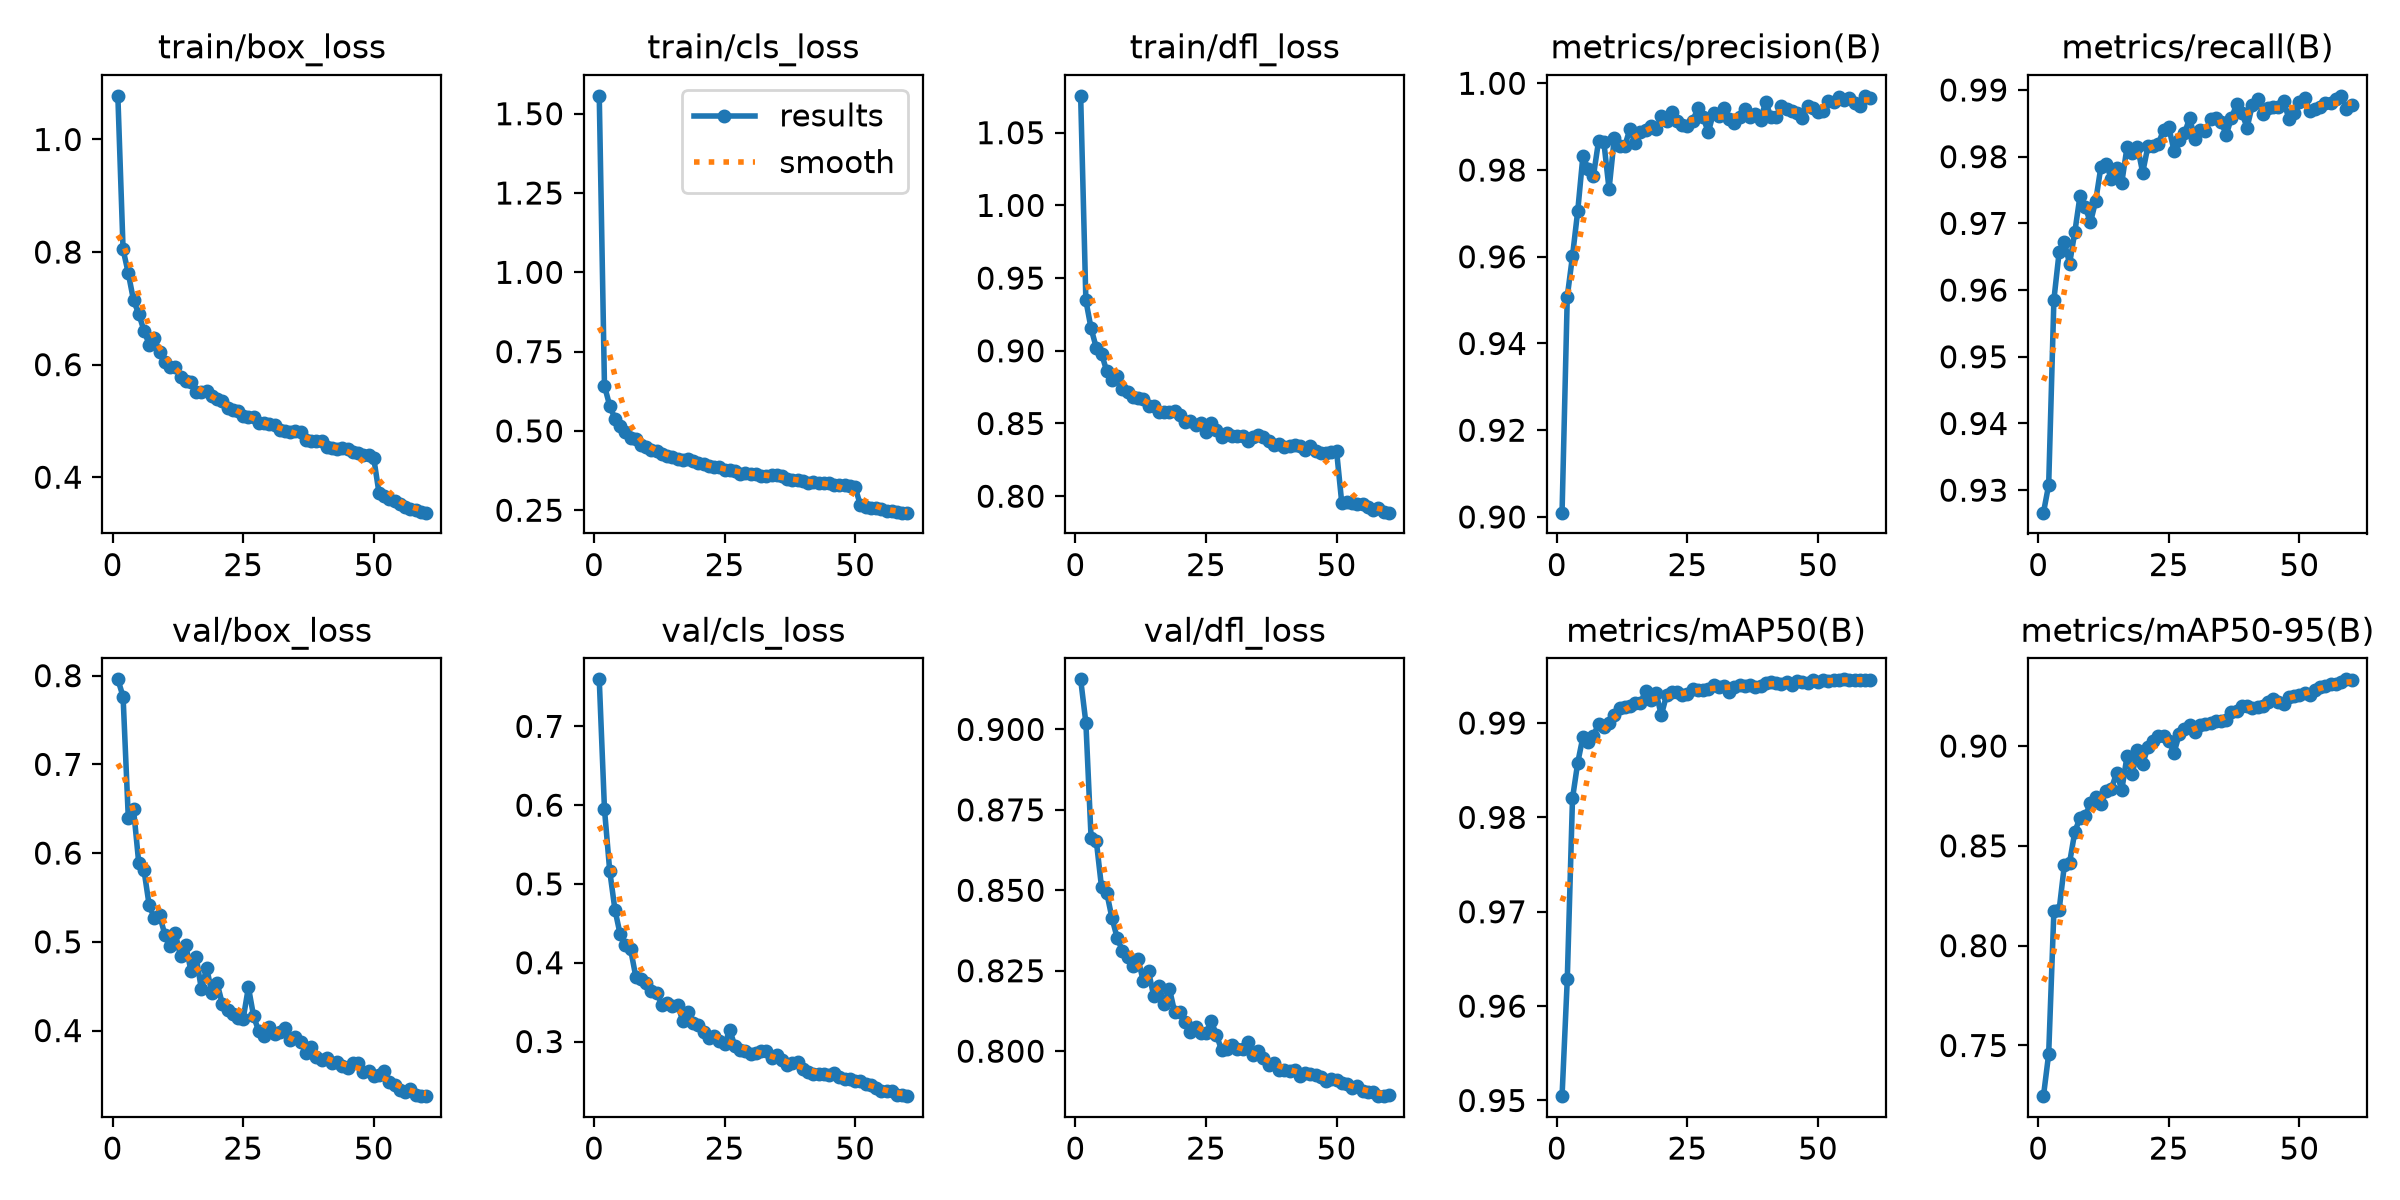
\includegraphics[width=\columnwidth]{training_curves.png}
\caption{Training and validation losses and metrics of the v2 detector over 60 epochs.}
\label{fig:training}
\end{figure}

\subsection{Threshold Tuning}
Five of the 13 tracer parameters (marked in Table~\ref{tab:params}) are tuned by coordinate
descent on the validation split only. The objective is
\begin{equation}
J = F_1^{\text{trans}} + 0.5\,E_{\text{struct}} + 0.25\,A_{\text{init}},
\end{equation}
where $F_1^{\text{trans}}$ is directed transition F1, $E_{\text{struct}}$ the share of
structurally exact graphs and $A_{\text{init}}$ initial-state accuracy. Detections are
computed once and only the deterministic reconstruction is re-run, so tuning is fast and
reproducible. In the recorded run the defaults scored $J=1.3931$ (transition F1 0.868,
structure-exact 0.55, initial accuracy 1.0 on the tuning sample) and no change improved
it, so the defaults were kept and \code{config/association.json} holds no overrides.

% =====================================================================
\section{Quantitative Evaluation}
\label{sec:results}
% =====================================================================

\subsection{Method}
All results are on the 360 held-out test diagrams. Predicted states are matched to ground
truth by bounding-box IoU $\ge 0.5$ using the Hungarian algorithm~\cite{kuhn} (SciPy
\code{linear\_sum\_assignment}), never by ID, because IDs only reflect detection order.
Transitions are compared through this matching. A transition counts as correct only if
both endpoints \emph{and} the direction are right. Metrics are micro-averaged, i.e.\
counts are summed over all diagrams before dividing:
\begin{equation}
P=\frac{TP}{TP+FP},\quad R=\frac{TP}{TP+FN},\quad F_1=\frac{2PR}{P+R}.
\end{equation}
Text is scored by exact match and by the character error rate
\begin{equation}
\text{CER}=\frac{\sum d_{\text{Lev}}(\hat{s}, s)}{\sum |s|},
\end{equation}
where $d_{\text{Lev}}$ is the Levenshtein distance~\cite{levenshtein}. \emph{Endpoint
accuracy} is the share of matched state pairs whose transition has the correct direction.
\emph{Graph exact (structure)} requires every state, transition, direction, initial and
final state to be correct; \emph{with labels} also requires every name and label to match
character for character. \emph{Code conformance} is the share of predicted graphs whose
generated code passes its full plan; a diagram with no detected states counts as a
failure.

\subsection{Detector Results}
On the test split the v2 detector reaches precision 0.994, recall 0.987, mAP@50 0.992 and
mAP@50--95 0.934 over 5108 objects (Table~\ref{tab:perclass}). States and final states are
nearly perfect. Arrowheads are the hardest class under the strict measure, dropping from
0.982 to 0.832: they are only a few pixels across, so a small box shift costs a lot of IoU.
The detector finds them but cannot place the box to the pixel. Arrowheads and initial
markers have the lowest recall, as small objects that resemble parts of arrows.

\begin{table}[t]
\centering
\caption{Per-class detection on the test split (v2 model)}
\label{tab:perclass}
\footnotesize
\begin{tabular}{@{}lrcccc@{}}
\toprule
\textbf{Class} & \textbf{Inst.} & \textbf{P} & \textbf{R} & \textbf{AP50} & \textbf{AP50--95} \\
\midrule
state          & 1128 & 1.000 & 1.000 & 0.995 & 0.995 \\
arrow          & 1268 & 0.991 & 0.984 & 0.994 & 0.949 \\
final\_state   &  154 & 0.998 & 1.000 & 0.995 & 0.995 \\
arrowhead      & 1268 & 0.986 & 0.968 & 0.982 & 0.832 \\
initial\_marker&  360 & 0.992 & 0.972 & 0.993 & 0.935 \\
label          &  930 & 0.998 & 0.999 & 0.995 & 0.897 \\
\midrule
\textbf{All}   & 5108 & 0.994 & 0.987 & 0.992 & 0.934 \\
\bottomrule
\end{tabular}
\end{table}

Fig.~\ref{fig:pr} shows the precision-recall curves. Raising the confidence threshold
trades recall for precision. At 0.90, recall falls from 0.99 to 0.70 while precision only
rises from 0.987 to 0.998. The best-F1 threshold is 0.63 (F1 0.991), against 0.989 at the
pipeline's threshold of 0.40, so F1 is flat over a wide range and the lower threshold
favours recall. A missed arrowhead only makes direction uncertain, and that is flagged
for review.

\begin{figure}[t]
\centering
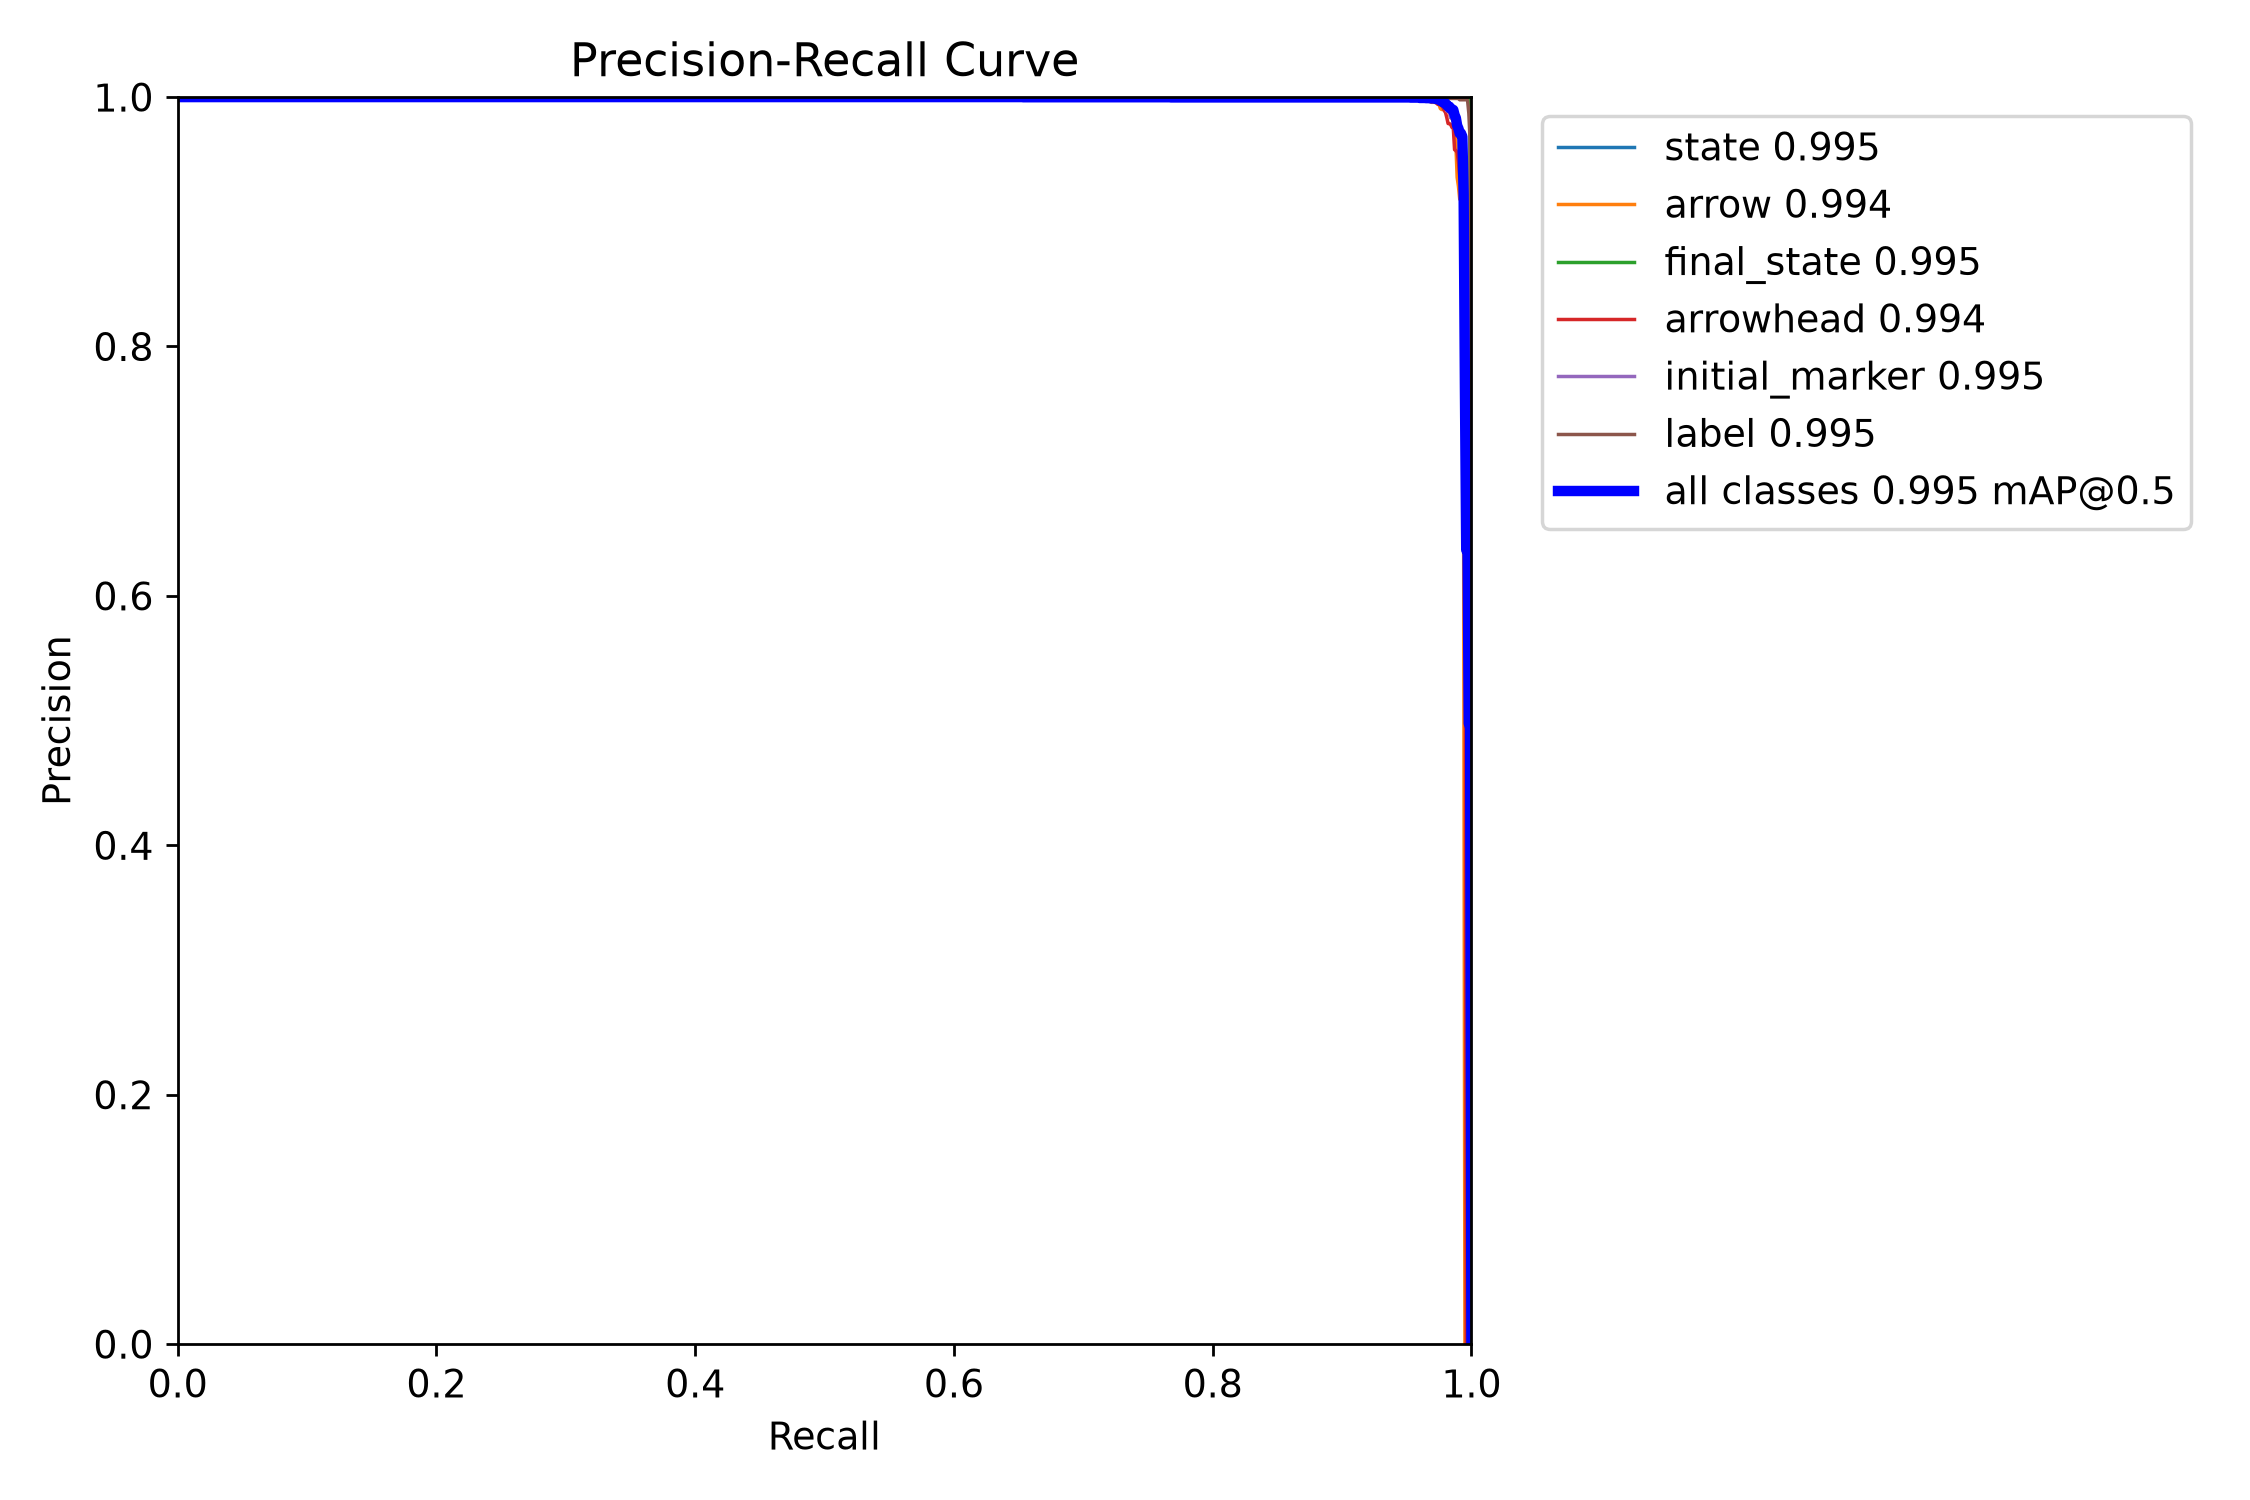
\includegraphics[width=0.95\columnwidth]{pr_curve.png}
\caption{Precision-recall curves of the v2 detector per class.}
\label{fig:pr}
\end{figure}

The confusion matrix (Fig.~\ref{fig:confusion}) is nearly diagonal. The off-diagonal
counts are between classes that look alike: 14 initial markers were predicted as arrows
(both are short arrows), 9 arrows as arrowheads, and 17 arrowheads and 4 arrows were
missed.

\begin{figure}[t]
\centering
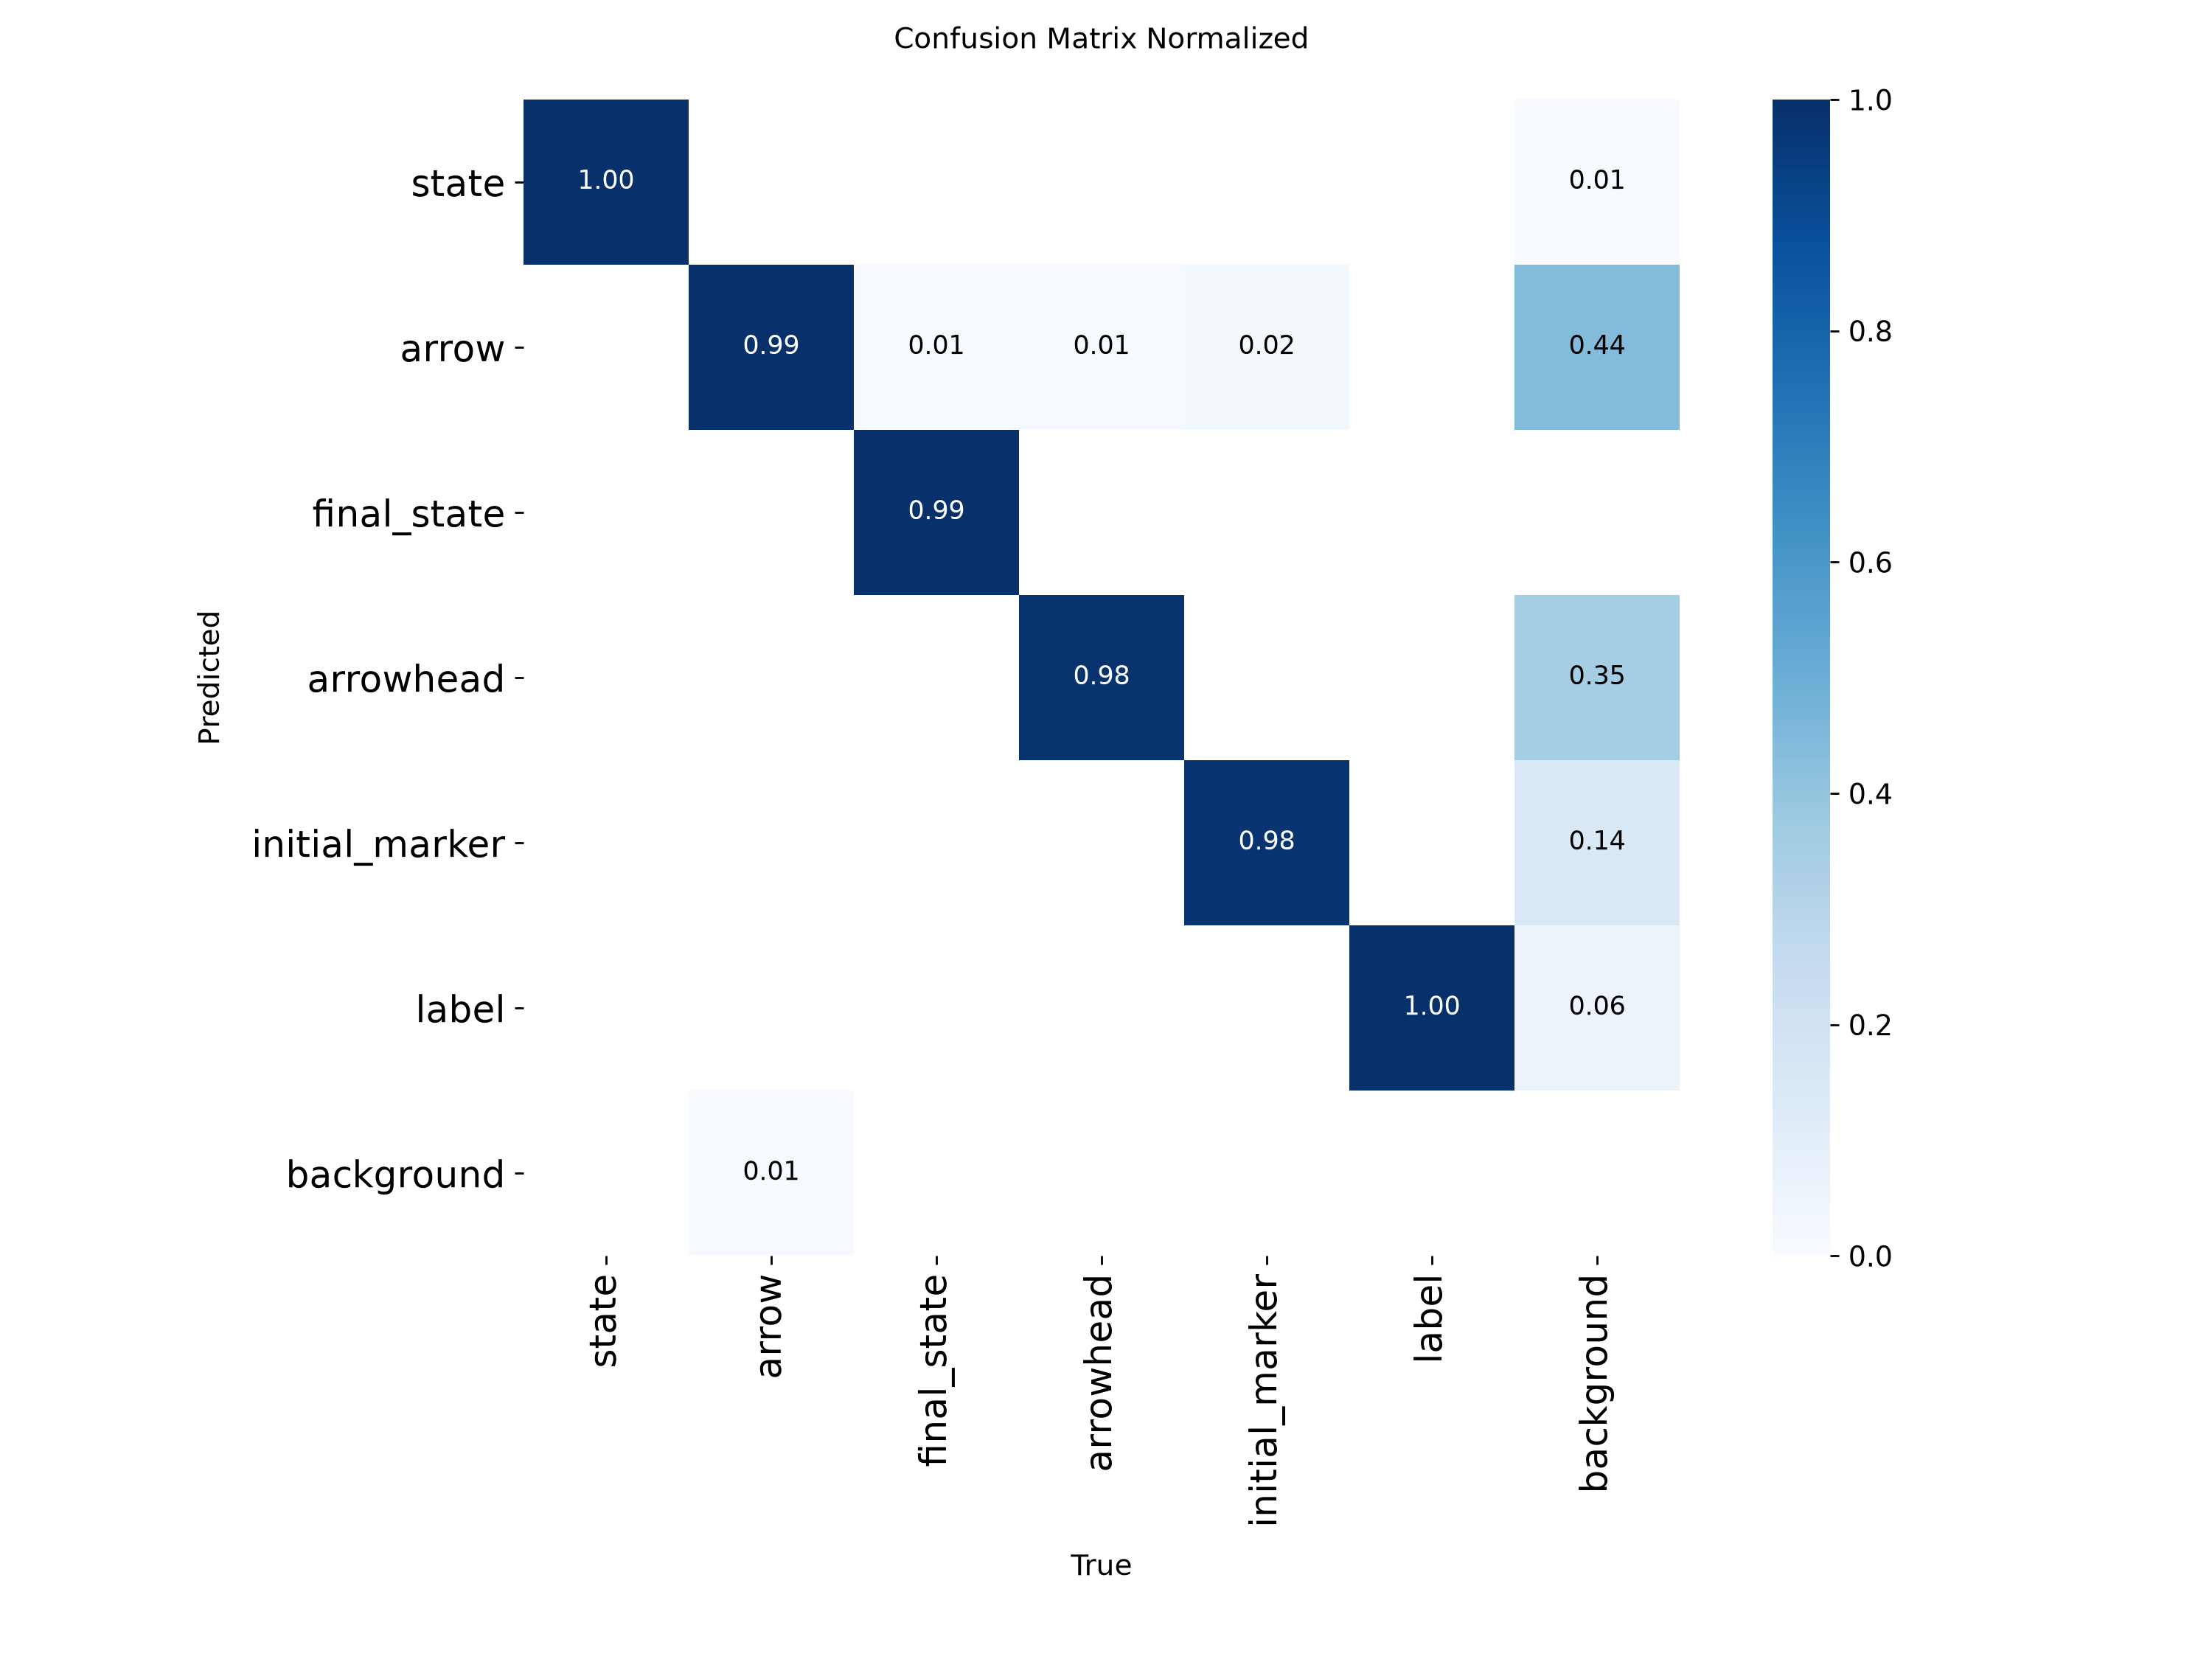
\includegraphics[width=0.92\columnwidth]{confusion_matrix.png}
\caption{Normalised confusion matrix of the v2 detector.}
\label{fig:confusion}
\end{figure}

\subsection{Graph Reconstruction: A/B/C Ablation}
Three configurations are compared:
\begin{itemize}
\item \textbf{A}: original pipeline. Two-class v1 model, box geometry, nearest-centre
association, no OCR.
\item \textbf{B}: v1 model with the new tracing, OCR and semantics. This isolates the
effect of the \emph{algorithm}.
\item \textbf{C}: retrained six-class v2 model with the new pipeline. This adds the effect
of better \emph{detection}.
\end{itemize}
Table~\ref{tab:ablation} gives the rates and Table~\ref{tab:counts} the underlying counts.

\begin{table}[t]
\centering
\caption{Graph reconstruction on 360 held-out diagrams}
\label{tab:ablation}
\footnotesize
\begin{tabular}{@{}lccc@{}}
\toprule
\textbf{Metric} & \textbf{A} & \textbf{B} & \textbf{C} \\
\midrule
State F1                    & 0.877 & 0.877 & \textbf{1.000} \\
Transition precision        & 0.282 & 0.696 & \textbf{0.950} \\
Transition recall           & 0.370 & 0.505 & \textbf{0.908} \\
Transition F1 (directed)    & 0.320 & 0.585 & \textbf{0.928} \\
Transition F1 (undirected)  & 0.486 & 0.717 & \textbf{0.957} \\
Endpoint accuracy           & 0.614 & 0.793 & \textbf{0.964} \\
Initial-state accuracy      & 0.000 & 0.519 & \textbf{0.983} \\
Final-state F1              & n/a   & 0.279 & \textbf{0.997} \\
\midrule
State OCR exact             & 0.000 & 0.835 & \textbf{0.847} \\
State OCR CER $\downarrow$  & 1.000 & 0.058 & \textbf{0.052} \\
Label OCR exact             & 0.000 & 0.214 & \textbf{0.654} \\
Label OCR CER $\downarrow$  & 1.000 & 0.617 & \textbf{0.228} \\
Event exact                 & 0.000 & 0.254 & \textbf{0.747} \\
\midrule
Graph exact (structure)     & 0.000 & 0.089 & \textbf{0.719} \\
Graph exact (with labels)   & 0.000 & 0.019 & \textbf{0.269} \\
Code conformance            & 0.994 & 0.994 & \textbf{1.000} \\
\bottomrule
\end{tabular}
\end{table}

\begin{table}[t]
\centering
\caption{Raw counts behind Table~\ref{tab:ablation} (360 test diagrams)}
\label{tab:counts}
\footnotesize
\begin{tabular}{@{}lrrr@{}}
\toprule
\textbf{Count} & \textbf{A} & \textbf{B} & \textbf{C} \\
\midrule
States: GT / predicted / TP & 1282/1212/1094 & 1282/1212/1094 & 1282/1282/1282 \\
Transitions: GT & 1268 & 1268 & 1268 \\
\quad predicted & 1660 & 920 & 1212 \\
\quad correct (directed) & 469 & 640 & 1151 \\
\quad correct (undirected) & 712 & 784 & 1187 \\
Final states: GT / pred / TP & 154/0/0 & 154/25/25 & 154/153/153 \\
Initial correct / 360 & 0 & 187 & 354 \\
Labels exact / total & 0/347 & 101/472 & 565/864 \\
State names exact / total & 0/1050 & 877/1050 & 1042/1230 \\
Graphs exact (struct.) & 0 & 32 & 259 \\
Graphs exact (full) & 0 & 7 & 97 \\
Code conformant / 360 & 358 & 358 & 360 \\
\bottomrule
\end{tabular}
\end{table}

\textbf{Interpretation.} Changing only the algorithm (A$\rightarrow$B) raises directed
transition F1 from 0.320 to 0.585, and changing only the detector (B$\rightarrow$C) raises
it to 0.928. Pipeline~A over-predicted, producing 1660 transitions for 1268 real ones, of
which only 469 were correct. B was cautious, with 920 predicted and 640 correct. C
predicted 1212 and got 1151 right. Of C's errors, 36 transitions had the right pair of
states but the wrong direction, 81 were missed or linked to the wrong state, and 25 were
spurious. Initial-state accuracy went from 0.000 to 0.983, and final states, never
detected by A, reach F1 0.997.

\textbf{Component versus task metrics.} The v1 detector already had a validation mAP@50 of
0.994, yet the graph-level transition F1 was only 0.32. A component metric can look
saturated while the task metric still has most of its headroom, so the task itself has to
be measured.

\textbf{Text.} Structure is strong: 72\,\% of graphs are structurally exact. Text is
weaker. State names have a CER of 0.052, but transition labels, which are small text on or
near lines and contain brackets and slashes, have a CER of 0.228 and 65\,\% exact match.
Since one wrong character fails a whole diagram, only 27\,\% of graphs are exact including
every label. This is why the editor exists and why low-confidence OCR is flagged.

\textbf{Code.} For every predicted graph in C (360/360), the generated code passed its
conformance plan. A and B each had two failures; by design, a predicted graph that is
empty or fails validation counts as non-conformant. Conformance shows that the code matches the \emph{graph}; whether the graph
matches the \emph{drawing} is measured by the reconstruction metrics.

% =====================================================================
\section{Qualitative Results}
\label{sec:qual}
% =====================================================================
Table~\ref{tab:hard} lists the hand-designed hard cases from the demo set and the
behaviour observed with the current system.

\begin{table*}[t]
\centering
\caption{Hard-case demo images and observed behaviour}
\label{tab:hard}
\footnotesize
\begin{tabular}{@{}L{3.6cm}L{6.2cm}L{6.8cm}@{}}
\toprule
\textbf{Image} & \textbf{Challenge} & \textbf{Observed result} \\
\midrule
\code{crossing\_edges.png} & Two diagonals cross in the middle & Idle$\rightarrow$Busy and
Wait$\rightarrow$Done (not Idle$\rightarrow$Done); the tracer goes straight through \\
\code{bidirectional\_and\_loop.png} & Two curved arrows between the same states, one each
way, plus a self-loop & \code{open}/\code{close} pair recovered with correct directions;
self-loop \code{tick} on Open \\
\code{arrow\_without\_head.png} & Line with no arrowhead & Edge drawn amber, dashed, with
``?''; Issues tab reports ambiguous arrowhead evidence and both directions \\
\code{dangling\_arrow.png} & Stroke ends in empty space & No transition invented; warning
that a state may be missing \\
\code{no\_initial\_marker.png} & No initial marker; End is a double ring & Warning asks
the user to mark the initial state; End recognised as final \\
\code{tcp\_handshake.png} & Network events, guards, actions, retry loop & 5 states,
6 transitions; self-loop \code{timeout [retries< 3] / retransmit}; DONE final \\
\code{net\_01\_photo.jpg} & Perspective, shading, low contrast & Structure mostly right;
state names misread (e.g.\ ``Seenngd nn'') --- domain gap \\
\bottomrule
\end{tabular}
\end{table*}

\subsection{Worked Example: TCP-style Handshake}
Fig.~\ref{fig:tcp} shows the TCP-style example. The pipeline detects 5 states and 6
transitions: \code{CLOSED} with the initial marker, \code{DONE} as a double-ring final
state, network events (connect, timeout, SYN-ACK, close, ACK) and a retry self-loop on
\code{SYN\_SENT}. The self-loop's label is parsed into event \code{timeout}, guard
\code{retries< 3} and action \code{retransmit}. The extra space in the guard is an OCR
slip that the user can fix in the editor. From the CLI:
\begin{itemize}
\item \code{generate} writes the code and reports \emph{38 conformance steps passed};
\item the exported test module runs \emph{15 passed};
\item \code{verify \dots{} connect SYN-ACK close ACK} gives the expected and actual
sequence S0$\rightarrow$S1$\rightarrow$S2$\rightarrow$S4$\rightarrow$S3 (CLOSED,
SYN\_SENT, ESTAB, FIN\_WAIT, DONE), \code{valid: true}.
\end{itemize}
With an API key, Gemini's explanation of ``What happens when the connection times out?''
correctly describes the retry guard: retransmit while retries $<3$, otherwise return to
CLOSED.

\begin{figure}[t]
\centering
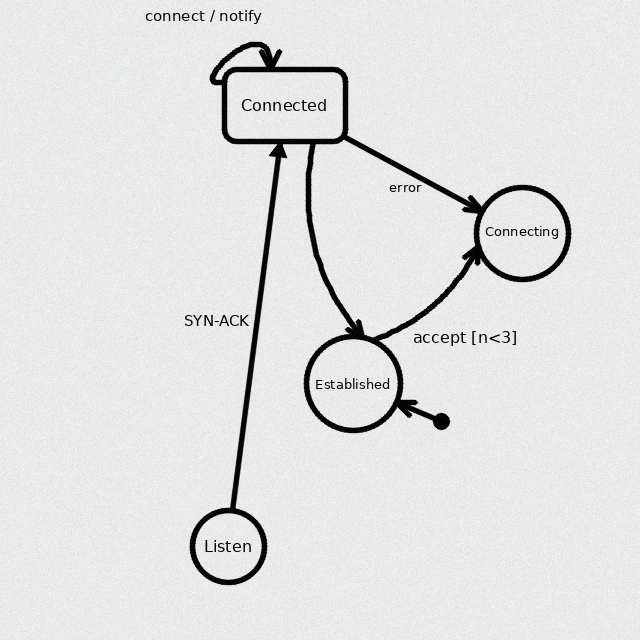
\includegraphics[width=0.95\columnwidth]{tcp_example.png}
\caption{TCP-style handshake example with network events, guards
(\code{[retries<3]}, \code{[retries>=3]}), actions, a retry self-loop and a final
\code{DONE} state.}
\label{fig:tcp}
\end{figure}

% =====================================================================
\section{Web Editor and Correction Loop}
\label{sec:editor}
% =====================================================================
\code{python main.py serve} starts the editor at \url{http://127.0.0.1:8000}. It uses only
the standard library, listens on localhost only, and checks upload size and image
signatures. Its parts are:
\begin{itemize}
\item \textbf{Source panel:} the image with detections and traced arrow paths overlaid.
\item \textbf{Graph panel:} zoom, pan, drag; double-click to add a state; \emph{Connect}
to draw a transition (the same state twice gives a self-loop); delete; undo/redo
(Ctrl+Z/Ctrl+Y); auto layout.
\item \textbf{Inspector:} rename, change type and shape, edit source/target, reverse or
confirm direction, edit event/guard/action, mark a network event, and edit network devices
and links (by form or by clicking two devices on the canvas).
\item \textbf{Issues tab:} validation errors, uncertainties and warnings; clicking one
selects the element.
\item \textbf{JSON tab:} editable and validated on the server before it replaces the
graph; e.g.\ a target \code{"S99"} is rejected with \emph{unknown state 'S99'}.
\item \textbf{Code tab:} generate (template or Gemini) and verify, with a ``stale'' badge
after later edits.
\item \textbf{Explain tab:} Gemini explanations and accept/reject suggestions.
\item \textbf{Export:} JSON, SVG, generated code and generated tests.
\end{itemize}

\textbf{Correction loop.} \emph{Save correction} stores a JSONL record with the image, raw
detections, predicted graph, corrected graph and a field-level diff.
\code{export-corrections} converts training-split records into YOLO labels and a dataset
file for fine-tuning, and \code{evaluate --corrections} measures a retrained model on
records saved as \emph{held-out}. Held-out records are never exported for training. No
real corrections have been collected yet, so no improvement from the loop is claimed.

% =====================================================================
\section{Software Engineering and Testing}
\label{sec:testing}
% =====================================================================

\subsection{Command-Line Interface}
Table~\ref{tab:cli} lists the commands of \code{main.py}.

\begin{table}[t]
\centering
\caption{CLI commands (\code{python main.py \dots})}
\label{tab:cli}
\footnotesize
\begin{tabular}{@{}L{2.4cm}L{5.4cm}@{}}
\toprule
\textbf{Command} & \textbf{Purpose} \\
\midrule
\code{IMAGE -o out.json} & Detect and reconstruct (\code{--diagram-type} state machine,
network or Petri net) \\
\code{analyze} & Reachability, cycles, dead ends, network events \\
\code{generate} & Code (template or \code{--backend gemini}) + conformance check, optional
\code{--tests} \\
\code{verify} & Full conformance or replay an event trace \\
\code{explain}, \code{suggest} & Gemini explanation / correction suggestions \\
\code{serve}, \code{edit} & Web editor (optionally bound to a file) \\
\code{evaluate} & Graph-level metrics on a split or on corrections \\
\code{compare} & Side-by-side table of evaluation results \\
\code{tune} & Tune tracer thresholds on the validation split \\
\code{export-corrections} & Corrections $\rightarrow$ YOLO training labels \\
\bottomrule
\end{tabular}
\end{table}

\subsection{Test Suite}
\code{python -m pytest -q} runs 71 tests in about 25\,s (70 test functions in 11 files,
Table~\ref{tab:tests}). Vision tests use programmatically drawn fixtures
(\code{tests/drawing.py}), Gemini tests use stubs so no key is needed, and the end-to-end
tests need the v2 weights.

\begin{table}[t]
\centering
\caption{Test coverage by file}
\label{tab:tests}
\footnotesize
\begin{tabular}{@{}lrL{4.4cm}@{}}
\toprule
\textbf{File} & \textbf{\#} & \textbf{Covers} \\
\midrule
\code{test\_pipeline.py} & 12 & Labels, network events, reconstruction, CLI, editor ops \\
\code{test\_contract.py} & 10 & Schema, round trip, v1.0 compat., semantic rules \\
\code{test\_vision.py} & 10 & Ink mask, direction, reversed arrows, loops, crossings,
double rings, ambiguity, label assignment \\
\code{test\_codegen.py} & 8 & Reference semantics, conformance, mutation, sandbox \\
\code{test\_evaluation.py} & 7 & Matching, CER, corrections, generator truth \\
\code{test\_ui\_api.py} & 7 & HTTP API, validation, uploads, error paths \\
\code{test\_gemini.py} & 6 & Contracts, dropped inventions, LLM tests \\
\code{test\_network.py} & 3 & Topology contract, OpenCV baseline \\
\code{test\_petrinet.py} & 3 & Token firing, disabled transitions \\
\code{test\_end\_to\_end.py} & 2 & Image $\rightarrow$ JSON $\rightarrow$ code
$\rightarrow$ traces \\
\code{test\_frontend.py} & 2 & Static pages and editor assets \\
\bottomrule
\end{tabular}
\end{table}

\subsection{Repository Structure}
\code{statemachine\_pipeline/} holds the modules of Table~\ref{tab:modules} plus
\code{models.py}, \code{schema.py}, \code{gemini.py}, \code{synthetic.py},
\code{evaluate.py}, \code{tune.py}, \code{corrections.py}, \code{ui.py} with
\code{static/}, \code{network.py}, \code{network\_cv.py} and \code{petrinet.py}.
Top-level scripts are \code{main.py}, \code{generate\_dataset.py},
\code{make\_test\_images.py} and \code{generate\_network\_diagrams.py}. Other folders are
\code{tests/}, \code{config/}, \code{legacy/}, \code{examples/tcp\_like/}, \code{demo/} and
\code{outputs/}. Weights, datasets, runs and generated test images are git-ignored and can
be regenerated (Appendix).

% =====================================================================
\section{Limitations}
\label{sec:limits}
% =====================================================================
\begin{itemize}
\item \textbf{Synthetic data only.} All measured numbers are on rendered diagrams. Photos
and hand drawings are out of distribution: expect lower detection quality and much lower
OCR accuracy. No real corrections have been collected or trained on yet.
\item \textbf{Association errors remain} for shallow crossings between arcs, arrows passing
under text and very small self-loops. They are often, but not always, flagged.
\item \textbf{Label OCR is the weakest stage.} A misread guard changes behaviour, so guards
should be reviewed before the code is used.
\item \textbf{Python only.} Gemini can emit other languages, but only Python is executed
and verified.
\item \textbf{Sandbox} isolation is at process level, not a container.
\item \textbf{Scope of conformance.} Tests check code against the graph, not the graph
against the drawing.
\item \textbf{Petri-net detection} needs a model that has not been trained.
\item \textbf{Unablated choices:} the horizontal-flip setting and the detector size were
not ablated.
\end{itemize}

% =====================================================================
\section{Lessons Learned}
% =====================================================================
\begin{enumerate}
\item \textbf{Measure the task, not the component.} A detector at mAP@50 $\approx0.99$ still
gave transition F1 0.32. Graph-level metrics revealed where the work was needed.
\item \textbf{Ablations make progress attributable.} Configuration B separated the
algorithmic gain from the detector gain.
\item \textbf{Ground truth by construction pays off.} Rendering diagrams from known graphs
made exact whole-graph evaluation and tuning possible.
\item \textbf{Saying ``unknown'' is a feature.} Explicit uncertainty turns silent errors
into review items.
\item \textbf{Keep LLMs out of the correctness path.} Restricting Gemini to explanation and
checked suggestions kept results reproducible and the system usable without a key.
\end{enumerate}

% =====================================================================
\section{Future Work}
% =====================================================================
In order of priority:
\begin{enumerate}
\item collect real hand-drawn and photographed diagrams, correct them in the editor, and
build a real-image training set and a held-out real test set;
\item fine-tune the detector on it and report real-image metrics;
\item replace or complement Tesseract with a handwriting-capable OCR model for labels;
\item reduce remaining association errors (shallow arcs, arrows under text, tiny loops)
and improve uncertainty coverage of these cases;
\item add more target languages under the same reference-based conformance check;
\item train the Petri-net detector and evaluate that mode;
\item move code execution into a container for untrusted use at scale.
\end{enumerate}

% =====================================================================
\section{Conclusion}
% =====================================================================
Over eight phases the project progressed from a box-only prototype with no notion of
direction, text or uncertainty to a complete image-to-verified-code system. On 360
held-out diagrams it recovers 93\,\% of transitions correctly with direction, gets 72\,\%
of graphs structurally exact, identifies initial and final states almost perfectly, and
produces code that passes its conformance tests for every predicted graph. The ablation
shows that the stroke-tracing algorithm and the richer detector each contribute about
half of the gain. The remaining gap is mainly label OCR and real-world images, and the
editor and correction loop are designed to close it.

% =====================================================================
\appendices
\section{Reproduction Commands}
{\footnotesize
\begin{verbatim}
# setup
python3 -m venv .venv && source .venv/bin/activate
pip install -r requirements.txt
cp .env.example .env     # GEMINI_API_KEY optional

# data and training
python generate_dataset.py --output dataset_v2 \
    --count 2400 --seed 7
yolo detect train data=dataset_v2/dataset.yaml \
    model=yolo11n.pt imgsz=640 epochs=60 \
    fliplr=0.0 project=runs/detect name=v2

# tuning and evaluation
python main.py tune --model runs/detect/v2/weights/best.pt
python main.py evaluate --split test --check-code
python main.py compare outputs/eval_*.json

# use
python main.py IMG.png -o out.json
python main.py generate out.json --tests test_out.py
python main.py serve
python -m pytest -q
\end{verbatim}
}

% =====================================================================
\begin{thebibliography}{10}

\bibitem{yolo11}
G.~Jocher and J.~Qiu, ``Ultralytics YOLO11,'' 2024. [Online]. Available:
\url{https://github.com/ultralytics/ultralytics}

\bibitem{tesseract}
R.~Smith, ``An overview of the Tesseract OCR engine,'' in \emph{Proc. 9th Int. Conf.
Document Analysis and Recognition (ICDAR)}, 2007, pp.~629--633.

\bibitem{opencv}
G.~Bradski, ``The OpenCV library,'' \emph{Dr. Dobb's J. Software Tools}, vol.~25, no.~11,
pp.~120--125, 2000.

\bibitem{gemini}
Gemini Team, Google, ``Gemini: A family of highly capable multimodal models,''
arXiv:2312.11805, 2023.

\bibitem{canny}
J.~Canny, ``A computational approach to edge detection,'' \emph{IEEE Trans. Pattern Anal.
Mach. Intell.}, vol.~PAMI-8, no.~6, pp.~679--698, 1986.

\bibitem{hough}
R.~O. Duda and P.~E. Hart, ``Use of the Hough transformation to detect lines and curves in
pictures,'' \emph{Commun. ACM}, vol.~15, no.~1, pp.~11--15, 1972.

\bibitem{uml}
Object Management Group, ``OMG Unified Modeling Language (UML), Version 2.5.1,'' 2017.

\bibitem{otsu}
N.~Otsu, ``A threshold selection method from gray-level histograms,''
\emph{IEEE Trans. Syst., Man, Cybern.}, vol.~9, no.~1, pp.~62--66, 1979.

\bibitem{clahe}
K.~Zuiderveld, ``Contrast limited adaptive histogram equalization,'' in \emph{Graphics
Gems IV}, P.~Heckbert, Ed. Academic Press, 1994, pp.~474--485.

\bibitem{kuhn}
H.~W. Kuhn, ``The Hungarian method for the assignment problem,'' \emph{Naval Research
Logistics Quarterly}, vol.~2, no.~1--2, pp.~83--97, 1955.

\bibitem{levenshtein}
V.~I. Levenshtein, ``Binary codes capable of correcting deletions, insertions, and
reversals,'' \emph{Soviet Physics Doklady}, vol.~10, no.~8, pp.~707--710, 1966.

\end{thebibliography}

\end{document}
